% !TeX program = pdflatex
% Companion note: one question connects Huddling, M5, the diatonic orbit, and convex energy.
% Author: Carles Marin Munoz (with AI assistance).
% Build twice with pdflatex; figure generation: python figs/huddling_figs.py from the project root.
\documentclass[11pt]{article}
\usepackage[T1]{fontenc}
\usepackage{lmodern}
\usepackage{amsmath,amssymb,amsthm,booktabs,graphicx}
\usepackage[hidelinks]{hyperref}
\usepackage{xurl}
\usepackage[table]{xcolor}
\usepackage[margin=1in]{geometry}
\usepackage{microtype}
\usepackage{placeins}
\usepackage{tikz}
\usetikzlibrary{arrows.meta,positioning,calc}
\definecolor{ctA}{HTML}{1B6F8C}
\definecolor{ctB}{HTML}{B5530F}
\setlength{\emergencystretch}{2em}
\setlength{\textfloatsep}{14pt plus 2pt minus 3pt}
\setlength{\floatsep}{12pt plus 2pt minus 3pt}
\setlength{\intextsep}{12pt plus 2pt minus 3pt}
\renewcommand{\topfraction}{0.95}
\renewcommand{\bottomfraction}{0.85}
\renewcommand{\textfraction}{0.05}
\renewcommand{\floatpagefraction}{0.85}
\raggedbottom
\newtheorem{theorem}{Theorem}
\newtheorem{lemma}{Lemma}
\newtheorem{proposition}{Proposition}
\newcommand{\lean}[1]{\texttt{#1}}
\newcommand{\Ztwelve}{\mathbb{Z}_{12}}
\newcommand{\Ahat}{\widehat A}
\newcommand{\question}[1]{\smallskip\noindent\textit{#1}\smallskip}
\newcommand{\orb}{\mathcal O_D}

\title{\bf Huddling, diatonic and pentatonic scales in $\Ztwelve$:\\
Fourier maxima and convex-energy minima\\ formalized in Lean 4}
\author{Carles Mar\'in Mu\~noz\thanks{Prepared with the assistance of artificial intelligence tools,
building on the author's earlier Lean development. The mathematical results are classical;
the author is responsible for the statements, attribution, and interpretation.
The formal artifact and its trust dependencies are described in Section~\ref{sec:checked}.}\\[3pt]
\normalsize Independent researcher\\
\normalsize \texttt{karlesmarin@gmail.com}}
\date{October 2026 \quad\textbullet\quad Version 1.1\\[3pt]\normalsize DOI: \href{https://doi.org/10.5281/zenodo.23123219}{10.5281/zenodo.23123219}\\\href{https://github.com/karlesmarin/music-math}{github.com/karlesmarin/music-math}}

\begin{document}
\maketitle
\begin{abstract}\noindent
The diatonic collection solves two optimization problems on the twelve pitch classes:
it maximizes the magnitude of the fifth discrete Fourier coefficient and minimizes an
all-pairs energy for every decreasing, discretely convex potential. We formalize the
connection in Lean~4. The route begins with the twelve-tone Huddling theorem: at each
cardinality, consecutive pitch classes maximize the first Fourier magnitude, with equality
exactly on their transposition orbit. Multiplication by five transports this maximum to
frequency five; at cardinality seven, the resulting orbit is precisely the diatonic orbit.
An Abel summation identity supplies the energy side. Under strict convexity and decrease,
the two equality classes coincide: for every seven-note set $A$,
$|\Ahat(5)|=2+\sqrt3$ if and only if $E_V(A)=E_V(D)$.
The contribution is a connected formalization of classical mathematics in $\Ztwelve$,
with exact algebraic comparisons, explicit equality conditions, and independently
reproducible cyclotomic checks. Two finite certificates use trusted compiled evaluation
(\lean{native\_decide}); the axiom audit makes these dependencies explicit.
A symbolic complement-energy identity transfers the
result to five-note pentatonic sets without another census. Homometry, tritone
transposition, and the parity coefficient connect the argument to the earlier notes.
\end{abstract}
\smallskip\noindent\textbf{Keywords:} Huddling lemma; diatonic scale; pentatonic scale; pitch-class sets;
discrete Fourier transform; maximal evenness; convex energy; Lean~4.

\section{Why do the same seven notes appear twice?}\label{sec:hook}

The seven white keys of the piano give the pitch-class collection
$D=\{0,2,4,5,7,9,11\}$, with $C=0$. On the twelve-position pitch-class clock they are spread
around the circle. Read in a different order, they form a consecutive chain of fifths.
These two views lead to two precise extremal properties of the same collection.

\question{P\textsubscript{0}. Why does this seven-note collection maximize a Fourier magnitude
and also minimize a repulsive pair energy?}

The historical routes to the question were different. Lewin's 1959 note on intervallic
relations~\cite{Lewin} supplied an early Fourier viewpoint. Clough and Douthett's 1991
study~\cite{CloughDouthett} developed maximal evenness as a property of scales.
Amiot recalls a more specific meeting of these ideas: the John Clough Memorial Days in
Chicago in July 2005, where Quinn's dissertation helped revive Lewin's Fourier approach
to chord quality~\cite{Amiot2009}. The occasion is a useful reminder that a change of
mathematical language can make connections in familiar musical material visible.

Douthett and Krantz connected maximally even configurations to interaction energies and
one-dimensional spin models~\cite{DK}. Amiot developed the Fourier characterization~\cite{Amiot2007}.
This note follows the connection between those viewpoints at one fixed scale. Its thread is
the diatonic collection throughout: first seen as a rearranged chromatic cluster, then as
a Fourier maximizer, and finally as an energy minimizer. The Lean statements make the
change of coordinates and the equality class explicit.

\section{The change of coordinates}\label{sec:coordinates}

For an unweighted set $A\subseteq\Ztwelve$, use the unnormalized DFT
\begin{equation}\label{eq:dft}
  \Ahat(t)=\sum_{a\in A}e^{-2\pi i at/12},\qquad
  S_t(A)=|\Ahat(t)|^2.
\end{equation}
In Lean, $A$ is a \lean{Finset (ZMod 12)} and the transform is Mathlib's
\lean{ZMod.dft} applied to its indicator. The complex-valued
\lean{Fourier.powerSpec} has real part $S_t(A)$; the bridge to the squared norm is
\lean{Huddling.powerSpec\_re\_eq\_norm\_sq}.
Transposition $T_sA=A+s$ changes phase and preserves $S_t$.

\question{P\textsubscript{1}. Which coordinates turn a consecutive chromatic cluster into
a diatonic collection?}

For a unit $u\in\Ztwelve^\times$, put $M_uA=\{ua:a\in A\}$. Reindexing the finite sum gives
\begin{equation}\label{eq:mtransform}
  \widehat{M_uA}(t)=\Ahat(ut).
\end{equation}
This is \lean{MTransform.Ahat\_mul}. Multiplication by five is its own inverse modulo twelve,
so it preserves cardinality and exchanges frequencies one and five. Five semitones is a
fourth, the reverse direction around the circle of fifths; this orientation has no effect
on the transposition class at issue here.
For $C_7=\{0,1,2,3,4,5,6\}$,
\[
 T_{11}M_5C_7=D,\qquad M_5D=T_7C_7.
\]
Both identities are checked on the same set definitions used in the theorems.

\begin{figure}[!htb]\centering
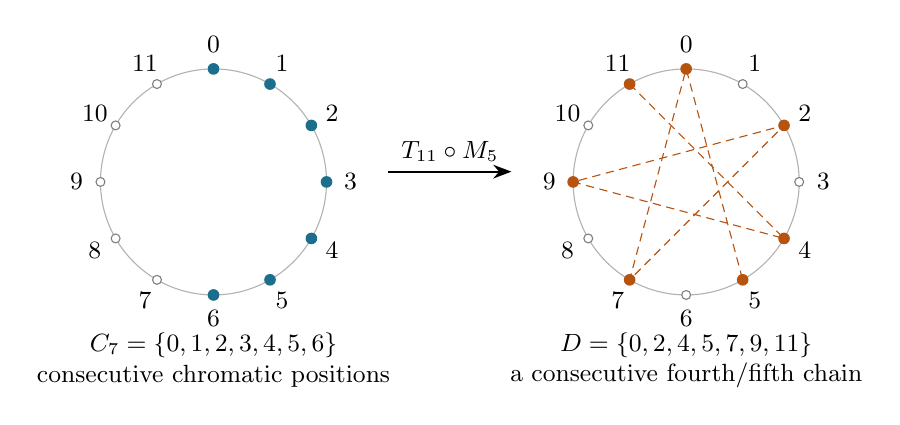
\begin{tikzpicture}[scale=0.87, every node/.style={font=\small}]
  \begin{scope}
    \draw[gray!60] (0,0) circle (1.65);
    \foreach \p in {0,...,11} {
      \coordinate (a\p) at ({90-30*\p}:1.65);
      \draw[fill=white,draw=gray] (a\p) circle (0.065);
      \node at ({90-30*\p}:2.00) {\p};
    }
    \foreach \p in {0,1,2,3,4,5,6} {\fill[ctA] (a\p) circle (0.085);}
    \node[align=center] at (0,-2.60) {$C_7=\{0,1,2,3,4,5,6\}$\\consecutive chromatic positions};
  \end{scope}
  \draw[-{Stealth},thick] (2.55,0.15) -- node[above,align=center] {$T_{11}\circ M_5$} (4.35,0.15);
  \begin{scope}[xshift=6.9cm]
    \draw[gray!60] (0,0) circle (1.65);
    \foreach \p in {0,...,11} {
      \coordinate (b\p) at ({90-30*\p}:1.65);
      \draw[fill=white,draw=gray] (b\p) circle (0.065);
      \node at ({90-30*\p}:2.00) {\p};
    }
    \foreach \p in {0,2,4,5,7,9,11} {\fill[ctB] (b\p) circle (0.085);}
    \draw[ctB,densely dashed] (b11)--(b4)--(b9)--(b2)--(b7)--(b0)--(b5);
    \node[align=center] at (0,-2.60) {$D=\{0,2,4,5,7,9,11\}$\\a consecutive fourth/fifth chain};
  \end{scope}
\end{tikzpicture}
\caption{The same seven positions in two coordinates. Filled nodes denote membership;
the dashed path on the right follows repeated addition of five, from $11$ to $5$.
The map permutes pitch classes and Fourier indices, carrying the first-frequency
cluster problem to the fifth-frequency diatonic problem.}
\label{fig:clocks}
\end{figure}

\section{What Huddling contributes}\label{sec:huddling}

The roots-of-unity lemma recorded by Amiot~\cite[Lemma~2]{Amiot2009} says that consecutive
roots maximize the magnitude of a sum of distinct roots. Here we certify its
twelve-tone instance and the complete equality class.

\begin{theorem}[Huddling in $\Ztwelve$]\label{thm:huddling}
For every $A\subseteq\Ztwelve$, with $k=|A|$ and $C_k=\{0,\ldots,k-1\}$,
\[
 S_1(A)\le S_1(C_k),\qquad
 S_1(A)=S_1(C_k)\ \Longleftrightarrow\ A=T_sC_k\text{ for some }s\in\Ztwelve.
\]
The same inequality and equality condition hold for Fourier magnitudes.
\end{theorem}

The formal proof reduces the comparison to an exact decidable order. If $i_j(A)$ counts
\emph{unordered} pairs at circular distance $j$, the autocorrelation/DFT bridge from
\lean{Fourier.lean} gives
\begin{equation}\label{eq:exact}
  2S_1(A)=P(A)+Q(A)\sqrt3,
\end{equation}
where
\[
 P(A)=2|A|+2i_2(A)-2i_4(A)-4i_6(A),\qquad
 Q(A)=2i_1(A)-2i_5(A).
\]
The factor at the tritone matters: the interval-vector convention here counts each
unordered tritone once. \lean{MTransform.psZ} represents the right-hand side in
$\mathbb Z[\sqrt3]$; \lean{powerSpec\_one\_re\_le\_iff} proves that its decidable
comparison agrees with real Fourier power. No rounded trigonometric values enter the proof.

The finite certificate bounds all $2^{12}=4096$ sets and identifies every equality witness.
The converse equality implication uses transposition invariance symbolically.
Table~\ref{tab:huddling} makes the finite scope and exact constants visible. At cardinalities
zero and twelve there is one maximizing set; at every intermediate cardinality there are
twelve, precisely the twelve distinct rotations of a proper consecutive arc.

\begin{table}[!htb]\centering
\rowcolors{2}{ctA!7}{white}
\begin{tabular}{@{}cccc@{}}\toprule
\rowcolor{ctA!22}
$k$ & Sets checked & $2S_1(C_k)$ & Maximizers\\\midrule
$0,12$ & $1$ each & $0$ & $1$ each\\
$1,11$ & $12$ each & $2$ & $12$ each\\
$2,10$ & $66$ each & $4+2\sqrt3$ & $12$ each\\
$3,9$ & $220$ each & $8+4\sqrt3$ & $12$ each\\
$4,8$ & $495$ each & $12+6\sqrt3$ & $12$ each\\
$5,7$ & $792$ each & $14+8\sqrt3$ & $12$ each\\
$6$ & $924$ & $16+8\sqrt3$ & $12$\\\bottomrule
\end{tabular}
\caption{The exact Huddling census. Complementary cardinalities share the nonzero-frequency
maximum, in agreement with the complement identity of \lean{Fourier.lean}.}
\label{tab:huddling}
\end{table}

\question{P\textsubscript{2}. What does the cluster maximum say about the seven white keys?}

Apply Theorem~\ref{thm:huddling} to $M_5A$ and use
Equation~\eqref{eq:mtransform}. For $|A|=7$ the result is
\begin{equation}\label{eq:diatonicmax}
 S_5(A)\le S_5(D)=7+4\sqrt3,
 \qquad |\Ahat(5)|\le2+\sqrt3.
\end{equation}
Equality holds exactly on
$\orb=\{T_sD:s\in\Ztwelve\}$.
The inversions of $D$ already belong to this orbit, so the transposition and $T/I$ descriptions
name the same twelve sets. This is why the word \emph{diatonic} is appropriate for this
Fourier extremum: the characterization singles out the collection up to transposition,
rather than selecting a tonic or one of its modal orderings.

\section{Why the energy selects the same collection}\label{sec:energy}

\question{P\textsubscript{3}. Can the equality class be recovered by measuring separation
between every pair of notes?}

Write $d(a,b)=\min((a-b)\bmod12,(b-a)\bmod12)$. For a real potential
$V:\{1,\ldots,6\}\to\mathbb R$, the all-pairs energy is
\begin{equation}\label{eq:energy}
 E_V(A)=\sum_{\{a,b\}\subseteq A}V(d(a,b))
       =\sum_{j=1}^{6}i_j(A)V(j).
\end{equation}
We call $V$ admissible when
\begin{equation}\label{eq:admissible}
 \Delta^2V(j):=V(j)-2V(j+1)+V(j+2)\ge0\quad(1\le j\le4),
 \qquad V(6)\le V(5).
\end{equation}
These hypotheses imply that $V$ is nonincreasing: its first differences are nondecreasing,
and the last is nonpositive. Strict admissibility means that all five displayed
inequalities are strict. No particular formula or positivity assumption on $V$ is required.

The proof reuses the symbolic engine in \lean{AllPairsEvenness.lean}.
For $|A|=7$, set $d_j=i_{j+1}(A)-i_{j+1}(D)$, $0\le j\le5$, and
\[
 H_j=\sum_{\ell=0}^{j}(j+1-\ell)d_\ell.
\]
Both sets have $\binom72=21$ pairs, so $\sum_{j=0}^5d_j=0$. Double Abel summation then gives
\begin{equation}\label{eq:abel}
 E_V(A)-E_V(D)=\sum_{j=0}^{3}H_j\Delta^2V(j+1)
                      +H_4\bigl(V(5)-V(6)\bigr).
\end{equation}
This identity is proved algebraically for arbitrary real $V$, independently of the census.
The finite input is that $H_0,\ldots,H_4\ge0$ for every seven-note set, and some $H_j>0$
outside $\orb$. On $\orb$ the whole interval vector agrees with that of $D$.
Equation~\eqref{eq:abel} therefore establishes a minimum for every admissible potential,
and identifies its equality class under the strict hypotheses.

\begin{theorem}[Diatonic energy minimum]\label{thm:energy}
For every admissible $V$ and every $A\subseteq\Ztwelve$ with $|A|=7$,
$E_V(D)\le E_V(A)$. If $V$ is strictly admissible, then
\[
 E_V(A)=E_V(D)\ \Longleftrightarrow\ A\in\orb.
\]
\end{theorem}

Strictness is essential to the equality statement. For the constant potential $V=1$, every
seven-note set has energy $21$, while only twelve maximize $S_5$. The weak minimum theorem
thus cannot be substituted for the strict uniqueness theorem in the connection below.

\section{The two questions have one equality class}\label{sec:connection}

We can now return to P\textsubscript{0}. Huddling identifies a consecutive arc; $M_5$ turns that
arc into the diatonic orbit; the Abel engine independently selects that same orbit.
The conjunction of the two characterizations gives the formal connection.

\begin{theorem}[Fourier--energy equivalence]\label{thm:connection}
For every strictly admissible $V$ and every seven-element $A\subseteq\Ztwelve$,
\[
 \boxed{\quad |\Ahat(5)|=2+\sqrt3\quad\Longleftrightarrow\quad E_V(A)=E_V(D).\quad}
\]
Both sides hold precisely for the twelve transpositions of $D$.
\end{theorem}
\begin{proof}
Equation~\eqref{eq:diatonicmax} identifies the left-hand equality class with $\orb$.
Theorem~\ref{thm:energy} identifies the right-hand equality class with $\orb$.
This is \lean{DiatonicExtremality.spectral\_energy\_equivalence}.
\end{proof}

For the concrete strictly admissible potential $V_0(j)=(7-j)^2$, the diatonic interval vector
is $(2,5,4,3,6,1)$ and its energy is $313$. Figure~\ref{fig:energy} shows all seven-note sets
in the two measurements. It illustrates the shared equality class; the theorem quantifies
over every strict admissible $V$, not just this plotted example.

\begin{figure}[!htb]\centering
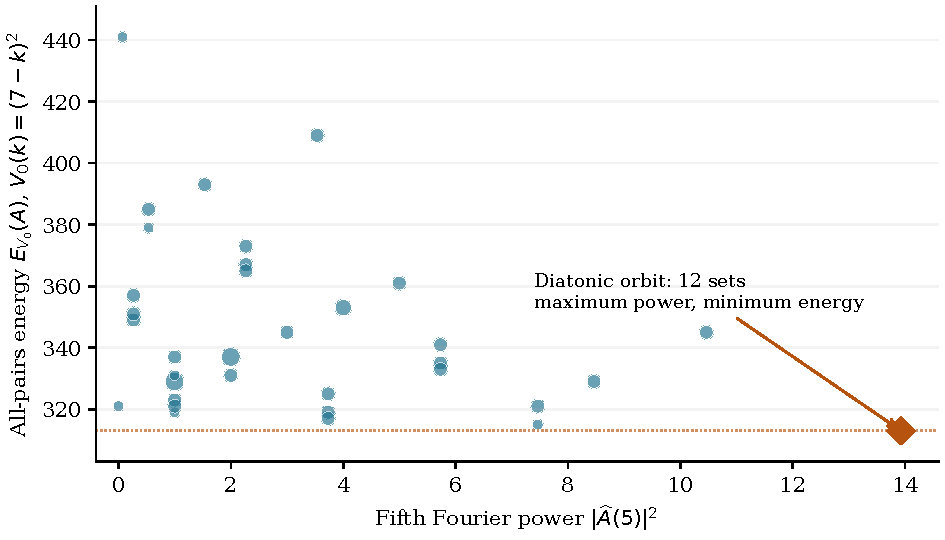
\includegraphics[width=0.94\linewidth]{figs/huddling_energy.pdf}
\caption{All $792$ seven-note sets, grouped into $34$ exact (Fourier power, energy) classes;
marker area increases with multiplicity. The diamond represents the twelve diatonic
transpositions, simultaneously at the largest $S_5$ and the smallest $E_{V_0}$.
Coordinates are computed exactly before conversion to plotting numbers.
Coincidence of the optimizers does not assert an ordering correspondence for every pair
of sets.}
\label{fig:energy}
\end{figure}

The previous note on the per-voice Fourier signature~\cite{Voice} used $a_5$ to measure
diatonic character in duration-weighted distributions. The present theorem explains the
extremal set interpretation of that name. Its domain is binary indicators at cardinality
seven: arbitrary duration weights require their own constraints, and the empirical
voice findings do not follow from this finite-set theorem.

\section{What happens to the five notes left over?}\label{sec:complements}

\question{P\textsubscript{4}. Do the black keys inherit both extremal properties of the white keys?}

Let $P=\{0,2,4,7,9\}$ be the anhemitonic pentatonic collection. The five black keys form
$D^c=T_6P$. Complementation is already part of the Fourier language of Note~2~\cite{Phase}:
for $t\ne0$, $\widehat{A^c}(t)=-\Ahat(t)$, so the magnitudes agree. This identity and the
complement closure of maximal evenness are classical~\cite{Amiot2006}.
The energy side requires keeping track of the unordered tritone convention. Our symbolic
proof first counts common tones under transposition:
\[
 |A^c\cap T_tA^c|+2|A|=12+|A\cap T_tA|.
\]
Consequently, $i_j(A^c)-i_j(A)=12-2|A|$ for $1\le j\le5$, and
$i_6(A^c)-i_6(A)=6-|A|$. Multiplying by the potential gives
\begin{equation}\label{eq:complenergy}
 E_V(A^c)-E_V(A)=(6-|A|)\left(2\sum_{j=1}^5V(j)+V(6)\right).
\end{equation}
No convexity is needed for this identity. It is the $C_{12}$ instance of the stronger
distance-degree-regular graph theorem of Bushaw, Cody, and Leffler~\cite[Theorem~3.5]{BCL}.
The new formal bridge exposes why the correction depends only on cardinality.
For a finite abelian group $G$ and an even potential $f(x)=f(-x)$, set
$E_f(A)=\frac12\sum_{a,b\in A}f(b-a)$. Translation makes every row sum equal to
$R_f=\sum_{x\in G}f(x)$, and hence
\begin{equation}\label{eq:groupcompl}
 E_f(A^c)-E_f(A)=\left(\frac{|G|}{2}-|A|\right)R_f.
\end{equation}
Equal-size sets therefore retain their energy gap under complementation; in particular,
complementation transports cardinality-constrained minimizers. For $G=\Ztwelve$,
$R_f=V(0)+2\sum_{j=1}^5V(j)+V(6)$. Our interval energy $E_V$ omits the diagonal;
setting $V(0)=0$ identifies its complement difference with
Equation~\eqref{eq:groupcompl}. A six-note set has the same energy as its complement
for every circular-distance potential. These are classical consequences of symmetry,
now linked to the exact twelve-tone convention in Lean.
For $|A|=5$, comparison with $D$ and $D^c=T_6P$ yields the exact gap identity
\[
 E_V(A)-E_V(P)=E_V(A^c)-E_V(D).
\]
Thus the five-note problem is obtained from the seven-note problem by a bijection,
with the energy difference preserved and the fifth Fourier coefficient negated.

\begin{theorem}[Pentatonic extremality]\label{thm:pentatonic}
For every five-element $A\subseteq\Ztwelve$, $|\Ahat(5)|\le2+\sqrt3$.
For every admissible $V$, $E_V(P)\le E_V(A)$. Under strict admissibility,
\[
 |\Ahat(5)|=2+\sqrt3\quad\Longleftrightarrow\quad
 E_V(A)=E_V(P)\quad\Longleftrightarrow\quad A=T_sP\text{ for some }s.
\]
\end{theorem}

The Lean proof uses the same two finite certificates as the diatonic result.
The complement bridge itself is symbolic. This also closes the opening piano image:
the white and black keys solve complementary problems, rather than providing unrelated
examples of regularity.

\section{What the earlier notes can now say}\label{sec:earlier}

\question{P\textsubscript{5}. Can a measurement that forgets phase still identify this scale?}

Note~2 studies homometry: equality of autocorrelation, equivalently of Fourier power.
Our bridge between its ordered interval counts and the unordered counts in
Equation~\eqref{eq:energy} proves
\[
 A\text{ and }B\text{ homometric}\quad\Longrightarrow\quad E_V(A)=E_V(B)
 \quad\text{for every }V.
\]
This is a consequence of the classical equivalent descriptions of homometry~\cite{AS}.
Moreover, homometry survives complementation: the autocorrelation identity above
changes every nonzero displacement count by the same cardinality-dependent constant.
Thus homometric $A,B$ also have homometric complements, whose pair energies agree
for every potential. This joins the phase question to the complement bridge without
an additional finite census.
For general sets, pair energies cannot recover phase or distinguish a nontrivial
homometric pair. At the diatonic extremum, however, spectral uniqueness implies
\[
 A\text{ homometric to }D\quad\Longleftrightarrow\quad A\in\orb.
\]
The equality class is rigid enough that forgetting phase leaves only the expected
transposition ambiguity. This corollary links the earlier phase question directly
to extremality; it is not claimed as a new mathematical theorem.

The same coordinate map also links the tritone of Note~1~\cite{Tritone} to the parity channel of
Note~4~\cite{Voice}. Since $5\cdot6=6\pmod{12}$,
\[
 \widehat{M_5A}(6)=\Ahat(6),\qquad M_5(T_6A)=T_6(M_5A).
\]
Thus $M_5$ exchanges the chromatic and diatonic Fourier coordinates while preserving
the sixth coefficient and commuting with the central tritone transposition. These
identities do not assert that a diatonic set has the 6-30 stabilizer, or explain a
duration-weighted corpus effect by themselves.

Finally, Note~3's Tonnetz spectrum~\cite{Tonnetz} contains $2\cos(\pi/12)$ as the fifth-frequency
magnitude of a generating \emph{triad}. Here the extremal \emph{seven-note scale}
has magnitude $2+\sqrt3$. The common Fourier coordinate connects the measurements;
their different cardinalities explain the different constants.

\section{What is machine-checked}\label{sec:checked}

\question{P\textsubscript{6}. Where are the links in this argument checked?}

\begin{figure}[!htb]\centering
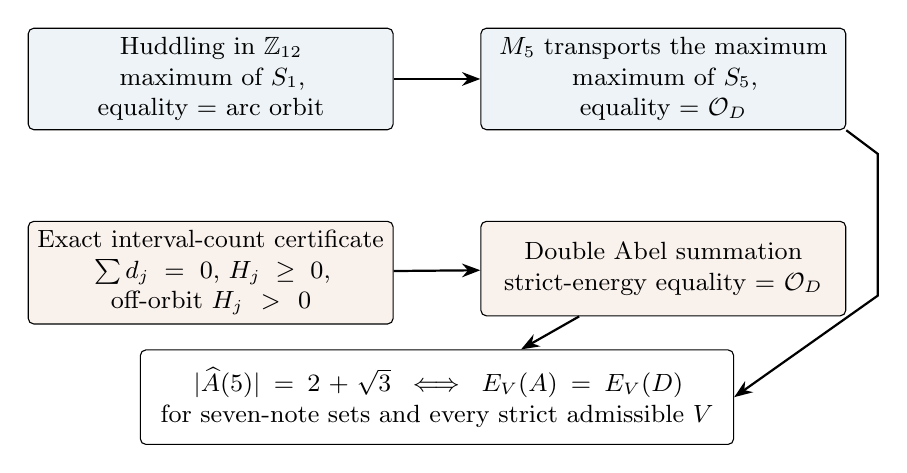
\begin{tikzpicture}[box/.style={draw,rounded corners=2pt,align=center,font=\small,
  text width=4.4cm,minimum height=1.2cm},arr/.style={-{Stealth},thick},node distance=1.15cm]
  \node[box,fill=ctA!8] (h) {Huddling in $\Ztwelve$\\maximum of $S_1$, equality = arc orbit};
  \node[box,fill=ctA!8,right=1.1cm of h] (f) {$M_5$ transports the maximum\\maximum of $S_5$, equality = $\orb$};
  \node[box,fill=ctB!8,below=of h] (e) {Exact interval-count certificate\\$\sum d_j=0$, $H_j\ge0$, off-orbit $H_j>0$};
  \node[box,fill=ctB!8,below=of f] (a) {Double Abel summation\\strict-energy equality = $\orb$};
  \node[box,text width=7.3cm,below=1.0cm of $(e)!0.5!(a)$] (c)
    {$|\Ahat(5)|=2+\sqrt3\ \Longleftrightarrow\ E_V(A)=E_V(D)$\\
    for seven-note sets and every strict admissible $V$};
  \draw[arr] (h)--(f);
  \draw[arr] (e)--(a);
  \draw[arr] (f.south east)--++(.4,-.3)--++(0,-1.8)--(c.east);
  \draw[arr] (a)--(c);
\end{tikzpicture}
\caption{The proof has two routes to the same equality class. The Fourier route uses
Huddling and the index permutation; the energy route uses finite integer counts and a
symbolic identity. The final theorem joins the routes rather than repeating two separate
optimization claims.}
\label{fig:proof}
\end{figure}

\begin{table}[!htb]\centering
\rowcolors{2}{ctA!7}{white}\footnotesize
\begin{tabular}{@{}p{0.47\linewidth}p{0.48\linewidth}@{}}\toprule
\rowcolor{ctA!22}
\textbf{Lean declaration} & \textbf{Role in the argument}\\\midrule
\lean{MTransform.Ahat\_mul} & Unit multiplication permutes Fourier indices.\\
\lean{MTransform.powerSpec\_one\_re\_le\_iff} & Exact $\mathbb Z[\sqrt3]$ comparison equals real power comparison.\\
\lean{Huddling.arc\_maximizes\_power}, \lean{arc\_unique} & All-cardinality Huddling inequality and equality class in $\Ztwelve$.\\
\lean{Huddling.fifth\_frequency\_unique} & Transports the complete equality characterization through $M_5$.\\
\lean{DiatonicExtremality.diatonic\_norm\_unique} & The seven-note maximum is $2+\sqrt3$, exactly on $\orb$.\\
\lean{AllPairsEvenness.abel\_bridge} & Symbolic double summation by parts, for arbitrary real potentials.\\
\lean{DiatonicExtremality.diatonic\_energy\_unique} & The same orbit is the strict-energy equality class.\\
\lean{DiatonicExtremality.}\newline\lean{spectral\_energy\_equivalence} & The joined Fourier--energy theorem.\\\bottomrule
\end{tabular}
\caption{The statements behind the narrative. Unqualified names in the Huddling row
belong to the same namespace.}
\label{tab:lean}
\end{table}

The file \lean{ExtremalityConnections.lean} adds
the connections in Sections~\ref{sec:complements}--\ref{sec:earlier}:
\begin{quote}\small
\lean{energy\_eq\_of\_homometric}, \lean{diatonic\_homometric\_iff};\\
\lean{m5\_preserves\_a6}, \lean{m5\_commutes\_tritone};\\
\lean{energy\_compl}, \lean{pentatonic\_energy\_gap};\\
\lean{pentatonic\_spectral\_energy\_equivalence}.
\end{quote}
The same file also proves \lean{homometric\_compl} and
\lean{energy\_compl\_eq\_of\_homometric}. The separate
\lean{TranslationInvariantEnergy.lean} proves the finite-group normal form
\lean{energy\_compl\_card} and \lean{energy\_gap\_compl}; its
\lean{PitchClassEnergy} specialization checks the row-sum formula,
the bridge to $E_V$, and complementary hexachord energy equality.

The development pins Lean~4.30.0-rc2 and Mathlib commit
\href{https://github.com/leanprover-community/mathlib4/tree/701fb6e9c3b9285968b375d19886bfc5ca134840}{\lean{701fb6e9c3b9}}
(the full revision is in \lean{lakefile.lean}).
The two new finite censuses use \lean{native\_decide} on exact arithmetic.
This adds trusted compiled-evaluation dependencies to the ordinary foundational axioms
\lean{propext}, \lean{Classical.choice}, and \lean{Quot.sound}; it is not kernel reduction
of the entire census. The explicit \lean{\#print axioms} output accompanies the build.
The symbolic Fourier transport and Abel identity use only the ordinary foundational
axioms; the final extremality theorem also inherits the two census dependencies.
The earlier \lean{AllPairsEvenness} file contains its own native census theorems,
but the new interface reuses its symbolic engine with the separately audited seven-note
certificate. No \lean{sorry}, \lean{admit}, or handwritten mathematical axiom is used.

Independent checks use two arithmetic routes: integer pairs $(P,Q)$ in
\lean{huddling\_verify.py}, and $\mathbb Q(\zeta_{12})$ with exact algebraic-real comparisons
in \lean{sage/huddling\_check.py}. The latter computes Fourier sums directly, independently
of Equation~\eqref{eq:exact}. Both verify all $4096$ sets and all $792$ seven-note
frequency-five cases. They support reproducibility; the Lean artifact specifies the theorem.

\section{Novelty, scope, and what this note does not claim}\label{sec:novelty}

Huddling, the Fourier index permutation, maximal evenness, and the energy viewpoint are
classical~\cite{Amiot2007,Amiot2009,CloughDouthett,DK}. The contribution here is their
connected formalization with the complete twelve-tone equality conditions, and the
explicit theorem joining the spectral and energy optimizers. The conjunction of
published equality-class characterizations is a corollary, not a new characterization.
Complement-energy transport is likewise covered in greater generality by Bushaw,
Cody, and Leffler~\cite[Theorems~2.16 and~3.5]{BCL}; the homometry and parity
connections follow from classical identities. It extends the earlier Fourier and
Abel machinery in this project.

The statement-level literature audit is recorded in
\lean{literature\_novelty\_2026-10-03.json}. It separates published theorems,
their consequences, and the question of proof-assistant implementation. The targeted
review establishes positive antecedents for the central mathematics; it does not
claim an exhaustive survey of every manuscript.

A dated overlap audit searched the October~3, 2026 Mathlib source snapshot
($8592$ Lean files) and the checked Prismriver snapshot ($35$ Lean files), inspected
their relevant Fourier and music modules, and ran indexed Huddling searches for
Lean, Coq/Rocq, Isabelle, and Agda. No matching formalization was located in those
sources. The audit records revisions, queries, and coverage in
\lean{formalization\_prior\_art\_2026-10-03.json}; a negative indexed search cannot
establish absence from every public or private codebase. Related Christoffel-word
results do exist in another Lean project and require a separate overlap review.

All Huddling statements in this note use $\Ztwelve$; the joined energy statements
fix cardinalities seven and five. We do not infer an arbitrary-universe formal theorem from this
finite census, or identify the energy optimizer with the fifth-frequency optimizer at
every other cardinality. The theorem concerns unweighted sets, not melodic order,
tonics, acoustic consonance, or the historical origin of the diatonic scale.

\section*{Coda: where the question leads}

The starting question has an exact answer: the seven white keys belong to one orbit
selected by two different objective functions, and $M_5$ connects the Fourier maximum
to a consecutive cluster. The resulting formalization leaves a concrete next question.

\question{Can the finite Huddling certificate be replaced by a structural Lean proof for
arbitrary roots of unity, retaining the full equality condition?}

The mathematical theorem already exists; the next task is to make its geometric argument
reusable in a proof assistant. Once that is available, the same coordinate change can be
studied for other cyclic universes. A further question is then precise rather than
metaphorical: which Fourier frequency and cardinality select the same orbit as a given
convex-energy problem? The present seven-of-twelve result supplies one checked instance
and a shared interface on which to build.

\section*{Data and code availability}
The source files \lean{Huddling.lean}, \lean{DiatonicExtremality.lean},
\lean{ExtremalityConnections.lean},
\lean{MTransform.lean}, \lean{Fourier.lean}, and \lean{AllPairsEvenness.lean} accompany
this note, together with the exact verification and figure scripts, the dated overlap
audit, and the pinned Lake configuration. The figure is reproducible from the code;
no corpus measurements are introduced in this note.

\FloatBarrier
\begin{thebibliography}{99}\small
\setlength{\itemsep}{3pt}
\bibitem{Lewin} D. Lewin, ``Re: Intervallic relations between two collections of notes,''
\emph{Journal of Music Theory} \textbf{3}(2) (1959), 298--301.
\href{https://doi.org/10.2307/842856}{doi:10.2307/842856}.
\bibitem{CloughDouthett} J. Clough and J. Douthett, ``Maximally even sets,''
\emph{Journal of Music Theory} \textbf{35}(1/2) (1991), 93--173.
\href{https://doi.org/10.2307/843811}{doi:10.2307/843811}.
\bibitem{Amiot2007} E. Amiot, ``David Lewin and maximally even sets,''
\emph{Journal of Mathematics and Music} \textbf{1}(3) (2007), 157--172.
\href{https://doi.org/10.1080/17459730701654990}{doi:10.1080/17459730701654990}.
\bibitem{Amiot2006} E. Amiot, ``Gammes bien r\'eparties et transform\'ee de Fourier discr\`ete,''
arXiv:math/0604210 (2006), Theorems~2, 6, and~7.
\url{https://arxiv.org/abs/math/0604210}.
\bibitem{Amiot2009} E. Amiot, ``Discrete Fourier Transform and Bach's Good Temperament,''
\emph{Music Theory Online} \textbf{15}(2) (2009).
\url{https://mtosmt.org/issues/mto.09.15.2/mto.09.15.2.amiot.html}.
\bibitem{DK} J. Douthett and R. Krantz, ``Maximally even sets and configurations: common
threads in mathematics, physics, and music,'' \emph{Journal of Combinatorial Optimization}
\textbf{14} (2007), 385--410.
\href{https://doi.org/10.1007/s10878-006-9041-5}{doi:10.1007/s10878-006-9041-5}.
\bibitem{BCL} N. Bushaw, B. Cody, and C. Leffler, ``Sets of vertices with extremal energy,''
arXiv:2407.18785 (2024), version~3 (2025), Theorems~2.16 and~3.5.
\url{https://arxiv.org/abs/2407.18785}.
\bibitem{AS} E. Amiot and W. A. Sethares, ``An algebra for periodic rhythms and scales,''
author manuscript (2009), Section~4.2.2.
\url{https://sethares.engr.wisc.edu/paperspdf/AlgofScales.pdf}.
\bibitem{Voice} C. Mar\'in Mu\~noz, ``The per-voice Fourier signature: the bass is the
spectrally purest voice,'' music-math series (2026).
\href{https://doi.org/10.5281/zenodo.20971090}{doi:10.5281/zenodo.20971090}.
\bibitem{Phase} C. Mar\'in, ``The phase taxonomy of pitch-class set invariants,''
music-math series, Note~2 (2026).
\href{https://doi.org/10.5281/zenodo.20826774}{doi:10.5281/zenodo.20826774}.
\bibitem{Tritone} C. Mar\'in, ``A tritone-centered self-duality: the set class 6-30 and its
order-12 neo-Riemannian dual,'' music-math series, Note~1 (2026).
\href{https://doi.org/10.5281/zenodo.20820962}{doi:10.5281/zenodo.20820962}.
\bibitem{Tonnetz} C. Mar\'in, ``The Tonnetz spectrum is the generating triad's Fourier balance
profile,'' music-math series, Note~3 (2026).
\href{https://doi.org/10.5281/zenodo.20862822}{doi:10.5281/zenodo.20862822}.
\bibitem{Mathlib} The Mathlib Community, \emph{Mathlib4}, with the \lean{ZMod.dft}
development by D. Loeffler. \url{https://github.com/leanprover-community/mathlib4}.
\bibitem{Prismriver} L. Aniva and C. Wang, \emph{Prismriver: Formalization of Music Theory
and Algorithmic Composition in Lean 4}, arXiv:2606.19936 (2026).
\url{https://github.com/lenianiva/Prismriver}.
\end{thebibliography}
\end{document}
